% Target: 35 pages
% Current: 3

\chapter{Adapters in Machine Translation}
\label{chap:adaptmt}
This chapter aims to study the impact of pre-trained models when fine-tuning machine translation models with adapters. Specifically, we are interested in understanding the contribution of good representation in the pre-trained language model to the adapters during the fine-tuning and the capability of adapters to perform with artificially degraded pre-trained models. We propose to use transformer-based architecture such as BERT and manually trained language models as the pre-trained weights in both encoder and decoder components while using adapters for the fine-tuning. To be more specific, we divide the experiments into four different areas:
\begin{itemize}
    \item Use BERT weights\footnote{We use publicly available BERT weights from Huggingface hub \url{https://huggingface.co}} as the pre-trained weights (\texttt{Pre-trained BERT}). We use this model as the baseline for the rest of our experiments.
    \item Use transformer architecture with BERT configuration and pre-train the models with MLM objective on IWSLT and WMT data (\texttt{Pre-trained Transformer}). This model configuration is used to pre-train the BERT models from scratch with data constructed from different domains and volumes. This is to understand the impact of different volumes and domains on the quality of the pre-trained models that will be fine-tuned with adapters in the later phase.
    \item Use transformer architecture with BERT weights as the pre-train weights where the weights are shuffled (\texttt{Pre-trained shuffled}). We use this configuration to understand whether the adapters can capture the importance of the original BERT weights and restore the performance even though the weights are not in the right place.
    \item Use transformer architecture with BERT configuration and entirely random weights as the pre-trained weights (\texttt{Pre-trained random}). We use this configuration as a complement of \texttt{Pre-trained shuffled} experiments to understand the impact of pre-trained models that contain relatively inferior knowledge than the original BERT model on the adapters when fine-tuned in the MT task.
\end{itemize}

\section{Experiments Setup}
\subsection{Language Model}
\label{ssec:langmodel}
\subsubsection{Dataset}
From \cite{devlin2018bert}, we understand that BERT is trained with billions of words from various sources and domains. However, we do not fully understand when we can stop adding sentences to the pre-training data so that we can reduce the hours of training the model. Furthermore, we do not know the impact of combining different domains in the pre-training data. For those reasons, we are reducing the scope of the pre-training data by restricting the creation of pre-training data only from machine translation datasets in two different domains and constructing the base models with different sizes of pre-trained data. We use WMT and IWSLT to construct the dataset as WMT and IWSLT contain different domains, and WMT has significantly larger sentences. Specifically, we construct three different datasets with different volumes:
\begin{enumerate}
    \item A standalone IWSLT. We use each of the languages in IWSLT as monolingual data used for fine-tuning.
    \item A combination of IWSLT and WMT data with a total of 500k sentences. Similar to the standalone IWSLT, except we add the WMT data as an addition to increase the volume of our pre-training data.
    \item A combination of IWLST and WMT data with 2 million sentences. The same as (2) but with larger volumes.
\end{enumerate}

The construction of the datasets was done with a simple approach by randomly selecting sentences from either dataset and combining them until we met the required number of sentences mentioned in the previous paragraph.

\subsubsection{Model}
To pre-train the model, we follow the work of \cite{devlin2018bert} by using the Masked Language Model (MLM) objective to train the model. Complete illustration can be found in \cref{img:mlmobj}. Essentially in every sentence, some words will be deleted, and the job of the model is to predict the missing words.

\begin{figure}[h]
    {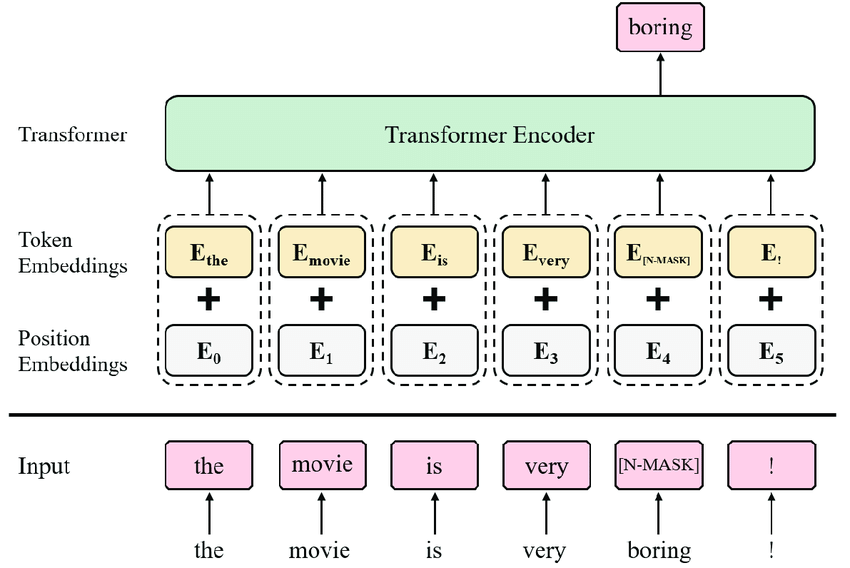
\includegraphics[width=0.95\textwidth]{img/mlm_obj.png}}
    \centering
    \caption{Illustration of the MLM objective during the pre-training. The illustration is reprinted from \cite{devlin2018bert}.}
    \label{img:mlmobj}
\end{figure}

The MLM is introduced as an alternative objective for the auto-regressive language model. The auto-regressive objective is inherently different from the MLM than in auto-regressive, where the models have to predict the word at step $t$ and the models only have the ability to look at the previous words ($t-1...0$) as the context.
One of the benefits of using this objective compared to the auto-regressive objective that is used in other models such as the GPT model \citewithpar{brown2020language,ratford2019language,radford2018improving} is that we can exploit the bidirectional context when training the model rather than only predicting the words from left-to-right.

We use the default BERT configuration from Huggingface to construct the model. A complete list of the hyperparameters can be found in \cref{tab:hyp}.

\begin{table}[]
    \begin{tabular}{@{}lccc@{}}
        \toprule
        \textbf{Name}                   & \textbf{En} & \textbf{De} & \textbf{Description}                                                                         \\ \midrule
        vocab\_size                     & 30522       & 31102       & \begin{tabular}[c]{@{}c@{}}Vocabulary size of the\\ BERT model\end{tabular}                  \\
        hidden\_size                    & 768         & 768         & \begin{tabular}[c]{@{}c@{}}Dimensionality for each\\ of the layers\end{tabular}              \\
        num\_hidden\_layers             & 12          & 12          & \begin{tabular}[c]{@{}c@{}}Number of hidden layers\\ in the transformer\end{tabular}         \\
        num\_attention\_heads           & 12          & 12          & \begin{tabular}[c]{@{}c@{}}Number of attention heads for\\ each attention layer\end{tabular} \\
        intermediate\_size              & 3072        & 3072        & \begin{tabular}[c]{@{}c@{}}Dimensionality of the\\ feed-forward layer\end{tabular}           \\
        hidden\_act                     & gelu        & gelu        & \begin{tabular}[c]{@{}c@{}}The activation function\\ within the layer\end{tabular}           \\
        hidden\_dropout\_prob           &
        0.1                             &
        0.1                             &
        \begin{tabular}[c]{@{}c@{}}The dropout probability\\ for all fully connected layers in\\ the embeddings, encoder,\\ and pooler\end{tabular}                \\
        attention\_probs\_dropout\_prob &
        0.1                             &
        0.1                             &
        \begin{tabular}[c]{@{}c@{}}The dropout ratio for the\\ attention probabilities\end{tabular}                                                                \\ \bottomrule
    \end{tabular}
    \caption{Transformer parameter for English based on \texttt{bert-base-uncased} German based on \texttt{bert-base-german-dbmdz-uncased}}
    \label{tab:hyp}
\end{table}

We train the model until convergence. The definition of convergence is to train the models for at least one day until the validation loss is no longer improving. We continue the training by loading the last checkpoint when the validation loss has not yet converged and still decreasing. Each language may end up converging in a different number of steps.

\subsection{Machine Translation}
\subsubsection{Dataset}
In machine translation experiments, there are several scenarios in which we use both WMT and IWSLT datasets. The IWSLT dataset is mainly used to fine-tune and evaluate the final model. The WMT, on the other hand, will be combined with IWSLT for training the baseline models. We use three different datasets for the experiments similar to the language model setup: IWSLT standalone, IWSLT + WMT (500k), IWSLT + WMT (2 million). To be more specific, we use the IWSLT standalone dataset for training, evaluation, and testing. For the rest of the datasets, we use them only for training, and we limit ourselves to the IWSLT data for evaluation and testing.

\subsubsection{Model}
We use the seq2seq architecture by \cite{vaswani2017attention}. The seq2seq architecture contains two different components, the encoder and the decoder. The details and an illustration of this architecture have been described in Chapter 1. The encoder and decoder use the same model and hyperparameters as described in \cref{ssec:langmodel}. The only modification made from the original language model is on the decoder side. We understand that on the encoder side, all the self-attention layers only refer to the neighbours of the current layer only for gathering the context. On the other hand, we need further context for the decoder by including the representation from the encoder as the extra features. For this reason, an extra component named \texttt{cross\_attention} layer is introduced in the decoder, and they are trained from scratch in any experiments.

\section{Experiments Results}
This section discusses the results obtained for machine translation tasks. First, in \cref{ssec:adaptcomp}, we conduct the comparative study of using adapters in different scenarios. Second, in \cref{ssec:randshuff}, we perform a study by replacing the BERT model with a different BERT version where the weights are shuffled. We continue the study of understanding the adapters' behaviour by replacing the pre-trained weights with a completely random set of weights and not using the BERT model. Finally, in \cref{ssec:randpre}, we perform experiments to understand the contribution of the total number of sentences used in the pre-training.

\subsection{Adapters Comparison}
\label{ssec:adaptcomp}
\subsubsection{Experiment Setup and Motivation}
In this section, we conduct experiments to understand the contribution of adapters by comparing trained and fine-tuned models with different sizes of datasets. The definition of the dataset is the same as have already explained in the previous section. The dataset is used for two different purposes:
\begin{itemize}
    \item Used by baseline model to train the model from scratch.
    \item Used for pre-training and later fine-tuned on IWSLT dataset.
\end{itemize}

\subsubsection{Experiment Results}
\begin{figure}[h]
    {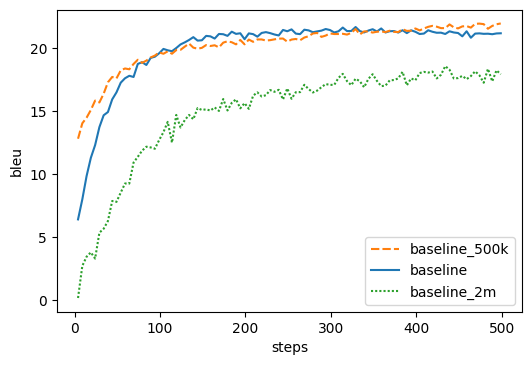
\includegraphics[width=0.95\textwidth]{img/baseline.png}}
    \centering
    \caption[Comparison between baseline models trained with different size of datasets.]{
        Comparison between baseline models trained with different size of datasets. \texttt{baseline} represents the model trained only using IWSLT; \texttt{baseline\_500k} represents the model trained using IWSLT and WMT with total of 500k sentence pairs; \texttt{baseline\_2m} represents the model trained using IWSLT and WMT with total of 2 million sentence pairs.}
    \label{img:basecomp}
\end{figure}

In this section, we compare the result of the baseline models with the fine-tuned models with adapters. From \cref{img:basecomp}, adding more data to the baseline models does not necessarily improve the performance. We suspect the models require more time to train to get the best final performance. There is a clear gap between \texttt{baseline\_2m} and the rest of the baseline models. \texttt{baseline} and \texttt{baseline\_500k} performs really well from the start while \texttt{baseline\_2m} lag behind. We suspect this is due to the effect of including more sentences from different domains. \texttt{baseline\_500k} is the best mix given the training time constraint. It balances the models to not overfitting in the intended domain and still benefits from out-of-domain data. \texttt{baseline\_2m} shows the impact on domain difference. It does not perform well on IWSLT, but it is growing and has a chance to improve its performance further. At a later stage, the \texttt{baseline\_2m} output would deserve manual evaluation because the lower bleu may not necessarily reflect a lower quality. We can see some of the results in \cref{tab:qtvout}.

To see the impact of including adapters, we compare the result on different sizes of pre-training data used for the base model. The base models are then fine-tuned with the adapters module on the IWSLT data. As we can see from \cref{img:adpcomp}, BERT achieves the best performance from the earlier steps compared to the rest of the pre-training size. In contrast to the baseline models, we see the benefit of adding more sentences to the pre-training. We can see the performance progression between the model that was trained using 500k data has lower performance than the one using 2 million data. On the other hand, models that only use IWSLT as the pre-training data suffer from performance degradation in the middle of the fine-tuning. We observed that this is due to the gradient explosion on the cross-attention layer. The IWSLT model eventually achieved similar performance to the 500k model in the later steps.
\begin{figure}[h]
    {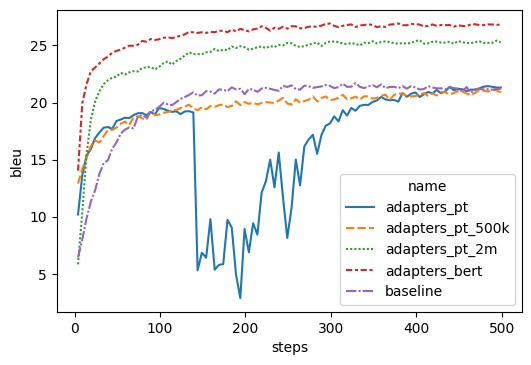
\includegraphics[width=0.95\textwidth]{img/adapterscomparison.png}}
    \centering
    \caption[Comparison between adapters pre-trained with different dataset sizes.]{
        % \XXX{Could you include baseline curve, too? This is rather important for comparison given the lack of the stopping criterion.}
        Comparison between adapters pre-trained with different dataset sizes. \texttt{baseline} represents the model trained only using IWSLT; \texttt{adapters\_pt} represents the model pre-trained only using IWSLT; \texttt{adapters\_pt\_500k} represents the model pre-trained using IWSLT and WMT with total of 500k sentence pairs; \texttt{adapters\_pt\_2m} represents the model pre-trained using IWSLT and WMT with total of 2 million sentence pairs; \texttt{adapters\_bert} represents the model that uses BERT weights.}
    \label{img:adpcomp}
\end{figure}

\begin{table*}[]
    \centering
    \begin{tabular}{@{}c@{}}
        \toprule
        \textbf{Random Weights + Adapters}                                                                                                                                                                                                             \\ \midrule
        \begin{tabular}[c]{@{}c@{}}\textbf{input}: wir tanzen im tempel und werden zu gott. \& quot ;\\ \textbf{prediction}: we \& apos ; re going to be able to become god. \& quot ;\end{tabular}                                                    \\ \midrule
        \begin{tabular}[c]{@{}c@{}}\textbf{input}: aber gleichzeitig hatten sie eine klare kenntnis des waldes, \\ die erstaunlich war.\\ \textbf{prediction}: but at the same time, they had a clear of the audience \\ who was amazing.\end{tabular} \\ \midrule
        \begin{tabular}[c]{@{}c@{}}\textbf{input}: es ist so wunderbar. ihr musst es beschutzen. \& quot ;\\ \textbf{prediction}: it \& apos ; s wonderful. you have to protect it. \& quot ;\end{tabular}                                             \\ \bottomrule
    \end{tabular}
    \caption{Prediction results from randomly set pre-trained model fine-tuned with adapters}
    \label{tab:qtrand}
\end{table*}

\subsection{Random and Shuffled Pre-training Weights}
\label{ssec:randshuff}
\subsubsection{Experiment Setup and Motivation}
To show to what extent the adapters can benefit from the pre-trained weights, we perform two different categories of experiments.
First, we conduct experiments where we shuffle the BERT weights. We separate the weights initialization into two approaches to perform the experiments:
\begin{itemize}
    \item We shuffled the weights from a column perspective. We shuffled the weights by preserving columns in all the weights matrices in the BERT network while keeping the row-wise order intact.
    \item We shuffled the weights from both column and row perspectives.
\end{itemize}

Second, we conduct experiments where we set random weights on all base network layers and treat them as the pre-training model. During the fine-tuning, we only update the adapter weights and keep the rest of the weights intact.

\subsubsection{Experiment Results}
We can see from \cref{img:shfrndcmp} the performance of the model that uses random weights as the pre-training model is more stable than the one using shuffled BERT weights. All shuffled BERT models suffer from gradient explosion similar to the IWSLT model we show in the previous section. Although the performance of the random model is still below the baseline model, it is interesting to see that only fine-tuning adapters and the cross-attention layer manage to achieve a reasonable BLEU score, considering that the pre-training models do not contain any meaningful information relative to the original BERT weights.
\begin{figure}[h]
    {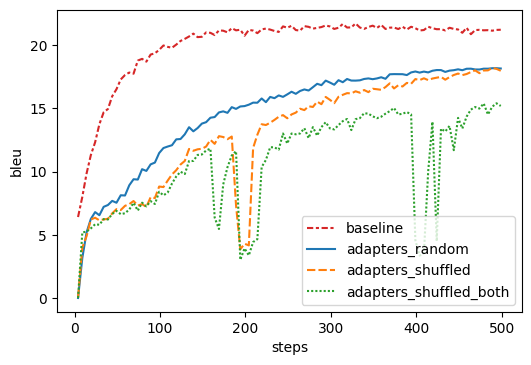
\includegraphics[width=0.95\textwidth]{img/randomshuffled.png}}
    \centering
    \caption[Comparison between adapters using shuffled BERT and random weights as the pre-trained models.]{Comparison between adapters using shuffled BERT and random weights as the pre-trained models. \texttt{baseline} represents the model trained only using IWSLT; \texttt{adapters\_random} represents the model pre-trained only using random weights; \texttt{adapters\_shuffled} represents the model pre-trained using column-wise shuffled BERT model; \texttt{adapters\_shuffled\_both} represents the model pre-trained using shuffled BERT model.}
    \label{img:shfrndcmp}
\end{figure}

Since we are relying on the base model with a random set of weights and with no further training, there is a possibility that our method may only work in a single random seed. To ensure a robust experiment, we repeat the random experiments ten times with ten different random seeds. We can see from the result in \cref{img:rndmseed} that all the random seed performs similarly to one another.

\begin{figure}[h]
    {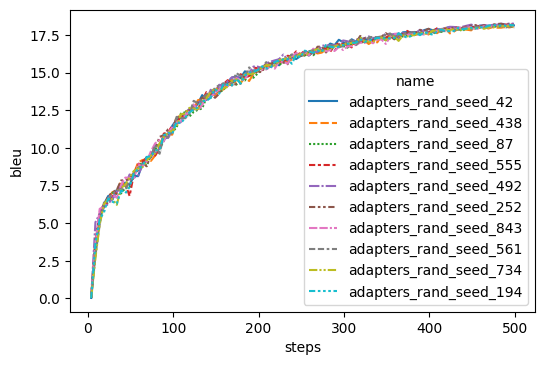
\includegraphics[width=0.95\textwidth]{img/adapter_random_multiseed.png}}
    \centering
    \caption{Comparison of different random seed for randomly set weights based models.}
    \label{img:rndmseed}
\end{figure}

\subsection{Random Pretraining vs. Out-of-Domain Data}
\label{ssec:randpre}
\subsubsection{Experiment Setup and Motivation}
In this experiment, we use the same setup as in \cref{ssec:adaptcomp,ssec:randshuff}. Specifically, we are interested in investigating the model's performance with the randomly set weights compared to the baseline model. We recall that we can gain a reasonable score from the previous experiments by using randomly set weights on the pre-trained model without further training. In this experiment, we are conducting further study to understand the performance relative to the baseline where the models were trained using a mix of WMT and IWSLT. This comparative study aims to understand whether we can benefit by only fine-tuning a small number of weights (adapters) versus training the whole transformer model with bigger data sizes.

\subsubsection{Experiment Results}
We further analyze the random weights by comparing the result with the best performing baseline and our pre-trained transformer models. From \cref{img:rndbslcmp}, we can see that the performance of the random model achieves a similar result to the baseline model that uses 2 million training sentence pairs. This tells us that training the whole model with bigger data does not necessarily improve the model's performance. It may need further tuning to gain the benefits of bigger data and bigger models. We can see the result of using random weights as a potential alternative for training the model with small data such as IWSLT. While the performance is still far from the baseline that is trained using only IWSLT data, this result shows that the base model's structure helps the adapter achieve a meaningful performance with very small weights required for the fine-tuning.

We perform a quick check on the output of the model in \cref{tab:qtrand}. From the first two lines, we can see that the model has difficulty capturing complex phrases. On the first row, the model missed \textbf{tanzen im tempel} which means \textbf{dancing in the temple}. For the second row, the model confuses \textbf{knowledge of the forest} and outputs \textbf{audience instead}. Furthermore, the model also does not translate the word \textbf{kenntnis} and makes the translation unclear since the object of the sentence is missing. Despite those mistakes, the model still can capture simple sentences, as shown in the third row. Another observation that we noticed in the generated output is the tokenization of \texttt{\&quot\;} and \texttt{\&amp\;}. Instead of being treated as a single token, the tokenizer treats the token as three different subword tokens. We notice that this is due to the unavailability of the aforementioned token in the pre-trained BERT vocabulary.

\begin{figure}[h]
    {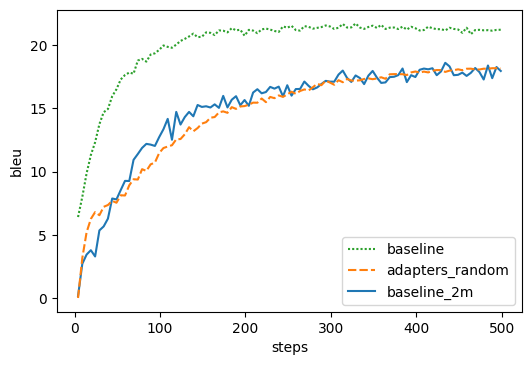
\includegraphics[width=0.95\textwidth]{img/random.png}}
    \centering
    \caption[Comparison between pre-trained random weights and baseline model.]{Comparison between pre-trained random weights and baseline model. \texttt{baseline} represents the model trained only using IWSLT; \texttt{baseline\_2m} represents the baseline model trained with a combination of IWSLT and WMT sentence pairs; \texttt{adapters\_random} represents the model pre-trained only using random weights; \texttt{adapters\_pt\_2m} represents the model pre-trained using IWSLT and WMT with total of 2 million sentence pairs; \texttt{adapters\_bert} represents the model that uses BERT weights}
    \label{img:rndbslcmp}
\end{figure}

\section{Qualitative Comparison}
\begin{sidewaystable*}
    \centering
    \begin{tabular}{|l|l|l|}
        \hline
        \multicolumn{1}{|c|}{\textbf{Baseline IWSLT}}                                                                                                                                                                                                                     &
        \multicolumn{1}{c|}{\textbf{IWSLT + WMT (total 2m)}}                                                                                                                                                                                                              &
        \multicolumn{1}{c|}{\textbf{BERT + Adapters}}                                                                                                                                                                                                                                \\ \hline
        \begin{tabular}[c]{@{}l@{}}\textbf{input}: erinnerst du dich an\\ den patienten\\ mit dem gereizten rachen? \\ \textbf{prediction}: do you remember\\ reading to the patients? on the\end{tabular}                                                                &
        \begin{tabular}[c]{@{}l@{}}\textbf{input}: erinnerst du dich an\\ den patienten\\ mit dem gereizten rachen? \\ \textbf{prediction}: do you remember\\ the patient with the tingling\\ revenge?\end{tabular}                                                       &
        \begin{tabular}[c]{@{}l@{}}\textbf{input}: erinnerst du dich an\\ den patienten\\ mit dem gereizten rachen? \\ \textbf{prediction}: remember the\\ patient with\\ the bruised remorse?\end{tabular}                                                                          \\ \hline
        \begin{tabular}[c]{@{}l@{}}\textbf{input}: großartig, sagte ich.\\ legte auf.\\ \textbf{prediction}: great, i said.\\ got up..\end{tabular}                                                                                                                       &
        \begin{tabular}[c]{@{}l@{}}\textbf{input}: großartig, sagte ich.\\ legte auf.\\ \textbf{prediction}: great, i said.\\ put on..\end{tabular}                                                                                                                       &
        \begin{tabular}[c]{@{}l@{}}\textbf{input}: großartig, sagte ich.\\ legte auf.\\ \textbf{prediction}: great, i said.\\ put it down.\end{tabular}                                                                                                                              \\ \hline
        \begin{tabular}[c]{@{}l@{}}\textbf{input}: - - aber in unserer\\ entdeckung der welt, haben\\ wir alle arten unterschiedlicher\\ methoden.\\ \textbf{prediction}: but in our discovery\\ of the world, we \& apos ;\\ ve got all sorts of different\end{tabular}  &
        \begin{tabular}[c]{@{}l@{}}\textbf{input}: - - aber in unserer\\ entdeckung der welt, haben\\ wir alle arten unterschiedlicher\\ methoden.\\ \textbf{prediction}: - - but in our discovery\\ of the world, we have\\ all kinds of different methods.\end{tabular} &
        \begin{tabular}[c]{@{}l@{}}\textbf{input}: - - aber in unserer\\ entdeckung der welt, haben\\ wir alle arten unterschiedlicher\\ methoden.\\ \textbf{prediction}: but in our discovery\\ of the world, we have\\ all sorts of different ways of doing\\ things.\end{tabular} \\ \hline
    \end{tabular}
    \caption{Prediction results from 1) Baseline model trained with only IWSLT data; 2) Pre-trained model with adapters where we pre-train the model with IWSLT and WMT with a total of 2 million pre-training data; 3) BERT with adapters.}
    \label{tab:qtvout}
\end{sidewaystable*}
We perform a sanity check to compare the generated results on some of our models. This sanity check checks the errors produced by the models on different techniques.
From \cref{tab:qtvout}, we can see that for the first example, none of the models managed to generate the correct result. However, BERT + adapters and 2 million pre-trained base models manage to generate the proper context where the result is still discussing \textbf{the patient}. The wrong part is when the model generates an incorrect translation regarding the patient's disease. The second example shows that the BERT + adapters create the correct and better output than the other models. The final example shows that BERT + adapters generate an interesting output where it manages to remove unimportant characters such as \texttt{--} and produce readable output. There may be a slightly different opinion on this example as the 2 million pre-trained base model generate a more concise output.

We also notice that the BERT base models have difficulties generating long sentences. The models always cut the translation short when an unavailable token such as \texttt{\&quot\;} appears in the sentence. To give a more explicit example, \cref{tab:errout} illustrates the significant difference in the outputs when the token \texttt{\&quot\;} is observed in the input. This shows that tokenization plays an essential role in the model where the tokens that are not available in the vocabulary list may affect the generated output.

\begin{table}[]
    \begin{tabular}{@{}l|l@{}}
        \toprule
        \multicolumn{1}{c}{\textbf{Input}}                                                                                                                                                          &
        \multicolumn{1}{c}{\textbf{Output}}                                                                                                                                                           \\ \midrule

        \begin{tabular}[c]{@{}l@{}}\& quot ; moneyball \& quot ; erscheint\\ bald und dreht sich um\\ statistiken und um diese zu nutzen\\ ein großartiges baseball team aufzustellen.\end{tabular} &
        \begin{tabular}[c]{@{}l@{}}\& quot ; devilball \& quot ; appears\\ soon, and it \& apos ;\end{tabular}                                                                                        \\ \midrule
        \begin{tabular}[c]{@{}l@{}}moneyball erscheint bald\\ und dreht sich um\\ statistiken und um diese zu\\ nutzen ein großartiges baseball\\ team aufzustellen.\end{tabular}                   &
        \begin{tabular}[c]{@{}l@{}}fatball soon appears and it\\ turns out statistics and\\ to use that to build a\\ great baseball team\end{tabular}                                                 \\ \bottomrule
    \end{tabular}
    \caption{The difference between similar input where the input on the first row containing extra token \texttt{\&quot\;}.}
    \label{tab:errout}
\end{table}